%%%%%%%%%%%%%%%%%%%%%%%%%%%%%%%%%%%%%%%%%%%%%%%%%%%%%%%%%%%%%%%%%%%%%%
% How to use writeLaTeX: 
%
% You edit the source code here on the left, and the preview on the
% right shows you the result within a few seconds.
%
% Bookmark this page and share the URL with your co-authors. They can
% edit at the same time!
%
% You can upload figures, bibliographies, custom classes and
% styles using the files menu.
%
%%%%%%%%%%%%%%%%%%%%%%%%%%%%%%%%%%%%%%%%%%%%%%%%%%%%%%%%%%%%%%%%%%%%%%

\documentclass[12pt]{article}

\usepackage{sbc-template}

\usepackage{graphicx,url}

%\usepackage[brazil]{babel}   
\usepackage[utf8]{inputenc}  

     
\sloppy

\title{Conceito, importância e aplicabilidade  port trás dos \\ modelo de Bancos de Dados Relacionais\\}

\author{Luca Ribeiro Schettino Regne\inst{1}}

\address{Departamento de Ciência da Computação -- \\
Pontifícia Universidade Católica de Minas Gerais (PUC-MG)\\
Belo Horizonte -- MG -- Brasil
}

\begin{document} 

\maketitle

\begin{resumo}
    Esse artigo tem como propósito principal narrar a história do Modelo de Bancos de Dados Relacionais bem como demonstrar o impacto benéfico, advinto do seu desenvolvimento, nos dias atuais. Questões como aplicabilidade, arquitetura, conceitos e problemas também serâo previamente abordados.
\end{resumo}


\section{Origem dos Bancos de dados Relacionais}
A palavra dado - do latim datum - pode ser definida como uma informação, documento ou testemunho e a partir dele é possível chegar ao conhecimento de algo. Por isso se torna imprescindível desenvolver cada vez mais maneiras eficientes de se ter o compartilhamento dos dados bem como seu armazenamento. Na internet chamamos de "Banco de Dados" os servidores ou aplicações utilizados para guardar e compartilhar grandes quantidades de informações.

A origem dos bancos de dados se deu na década de 60 quando a IBM (International Business Machines) - empresa voltada à informática - iniciou pesquisas e investiu fortemente nos servidores que posteriormente seriam utilizados por quase todas as aplicaçoes virtuais para armazenar grandes quantidades de informações. Diversos modelos surgiram neste mesmo período, dentre eles os modelos hierárquico e rede.

Edgar Frank "Ted" Codd - um dos pesquisadores da companhia - publicou,  em junho de 1970,  um artigo intitulado "A Relational Model of Data for Large Shared Data Banks", marcando o início do modelo relacional de armazenamento de dados.  Nesse modelos os dados são estruturados usando relações ou estruturas matemáticas semelhantes a grades que têm colunas e linhas semelhante a uma tabela.

No seu artigo era apresentado uma forma de usuários sem conhecimento técnico armazenarem e extraírem grandes quantidades de informações de um banco de dados. Este artigo motivou cientistas de todo o mundo a aprofundarem nos banco de dados relacionais, com o propósito de concretizar o, até então teórico, de modelo de Ted Codd.

Esse grande impulso tornou possível o desenvolvimento do que hoje conheçemos como SQL ou "Structured Query Language", que viria a ser desenvolvido no final da década de 70 juntamente com o "System R". Embora o sistema não tenha sido bem sucedido comercialmente, serviu de base para o desenvolvimento dos bancos de dados seguintes que se utilizaram da mesma linguagem de pesquisa declarativa, o SQL.

\section{SQL ou Structured Query Language}

Embora o SQL tenha sido originalmente criado pela IBM, no mesmo periodo diversos outros cientistas se propuseram a desenvolver outras linguagens, que apesar das diferneças tinham como propósito o mesmo: manipular os dados com a metodoliga Relacional. Em 1986 e 1987, respectivamente, foram desenvolvidas pela American National Standards Institute (ANSI) e pela International Organization for Standardization (ISO) padrões para a linguagem de pesquisa.

Após as padronizações ainda ocorreram outras revisões nos anos de 1992, 1999 e 2003 gerando as versões SQL-92, SQL:1999 (SQL3) e SQL:2003, respectivamente. Dentre os avanços produzidos entre elas podemos citar como funcamentais os implementados na versão do final da década de 90, sendo o uso de expressões regulares de emparelhamento, queries recursivas e gatilhos (triggers). Além disso, houve uma adição controversa de tipos não-escalados e algumas características de orientação a objeto. No SQL:2003 foram introduzidos características relacionadas a linguagem de marcação com o Extensible Markup Language (XML), tal como padronizações para colunas com valores de auto-generalização.

\section{SQLite}

Embora tenha surgido para armazenar grandes quantidades de dados um dos problemas gerado pelos banco de dados relacionais foi o consumo de muito recurso computacional mesmo quando não eram necessários armazenar muitas informações. Com o intuito de solucionar a problemática citada foi desenevolvido, em 17 agosto de 2000 pelo D. Richard Hipp usando a linguagem de programação C, o SQLite.

SQLite é uma biblioteca que implementa um banco de dados SQL embutido ao servidor,s endo assim não seria necessário executar um processo SGBD separado. A biblioteca permite escrever diretamente em um arquivo do disco os dados e posteriormente consultá-las para fornecer as informações para as demais aplicações.

\section{Aplicabilidade}

Imagine que um site está sendo desenvolvido para uma universidade e nele haverá um portal onde alunos e professores poderão registrar informações referentes a ementa e a grade curricular, tal como, resultados semestrais, notas e atividades. Para realizar a implementação desse site será necessário um banco de dados e devido a simplicidade do SQLite trataremos nos tópicos a seguir a aplicabilidade do SQLite nesse específico, porém usual, problema de arquitetura de banco de dados.

\subsection{Modelagem}

A fase mais importante e crítica na criação de um banco de dados é a sua modelagem. Essa etapa precede a implementalção da tecnologia e visa definir de maneira clara e sucinta seus requisitos funcionais - próprosito para os banco de dados e restrições de implementação - bem como lógicos - tipo dos dados (inteiro, caracter, booleano, etc), relações entre os dados e casos de interdepênceia, etc.

\subsubsection{Modelo Conceitual}

No Modelo Conceitual são mapeados as relações entre as informações do sistema. Geralmente, são feitoscom auxílio de diagramas de relacionamento, que descrevem ded maniera visual os atores envolvidos. 

Em muitos casos é utilizado a linguagem UML — Unified Modeling Language, para criação desse modelo.A partir dele é possível representar, em forma de entidades e relacionamentos, o que serão as tabelas e colunas bem como seus relacionamentos.

Para simplificação, supomos que nosso banco de dados deva ter a capacidade de registrar discentes e docentes, sendo que ambos tenham campos para armazenar o nome e a matrícula da instituição. Além disso, podemos resgistrar no primeiro o curso em andamento e no segundo a matéria conduzida.

Podemos registrar em uma terceira tabela o curso com os campos código, nome e lista de matérias. Essse ultimo pode referenciar outra tabela: a de matéria, que deve conter também nome e código além de uma carga horária.

Após essa definição teremos o seguinte modelo conceitual apresentado, a seguir:
\begin{figure}[ht]
\centering
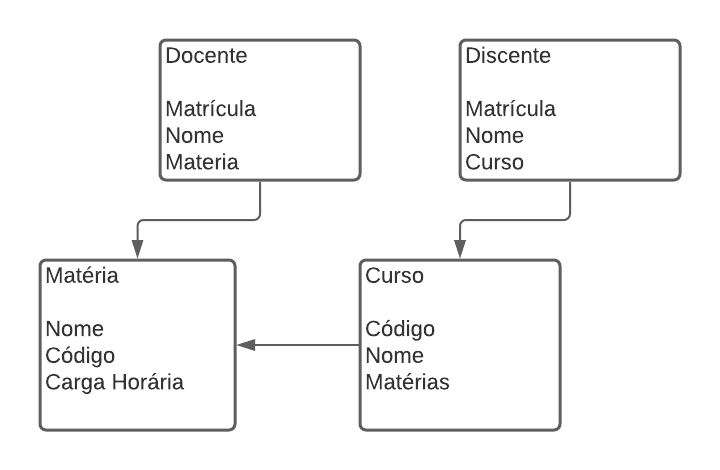
\includegraphics[width=1\textwidth]{Modelo_Conceitual.png}
\caption{Modelo conceitual.}
\label{fig:ModeloConceitual}
\end{figure}

\subsubsection{Modelo Lógico}

Na elaboração do Modelo Lógico são introduzidos conceitos primordiais apra criação do banco de dados, como as chaves primárias: valores únicos usados para identificar determinada coluna em uma tabela.

Na prática, podemos definir na nossa modelagem os respectivos códigos de matrícula como chaves primárias dos discentes e docentes e para as matérias e cursos um código que será um valor inteiro. 

\begin{figure}[ht]
\centering
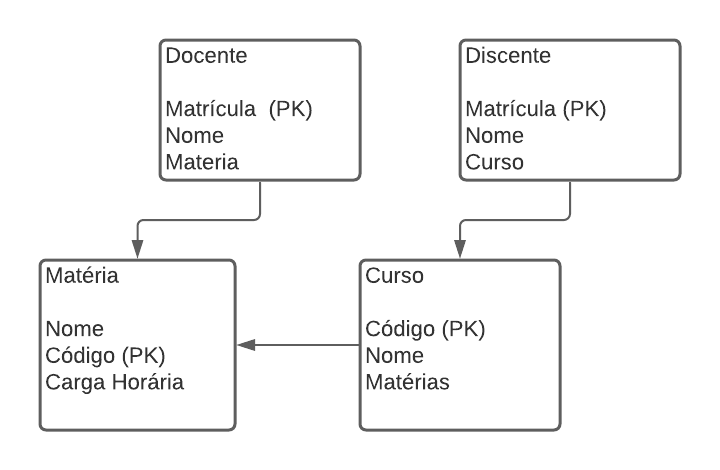
\includegraphics[width=.8\textwidth]{Modelo_Logico.png}
\caption{Modelo lógico.}
\label{fig:ModeLogico}
\end{figure}

\subsubsection{Modelo Físico}

Na etapa de definição do Modelo Físico são definidos detalhes técnicos do projeto como qual o SGBD utilizar e quais serão os tipos de dados utilizados para cada campo, em casos de strings são definidos a quantidade de caracteres e em float as casas decimais. Nessa fase também ocorre a implementação de scripts em código SQL que vai gerar a base de dados.

Definimos o modelo final conforme a imagem apresentada a seguir:

\begin{figure}[ht]
\centering
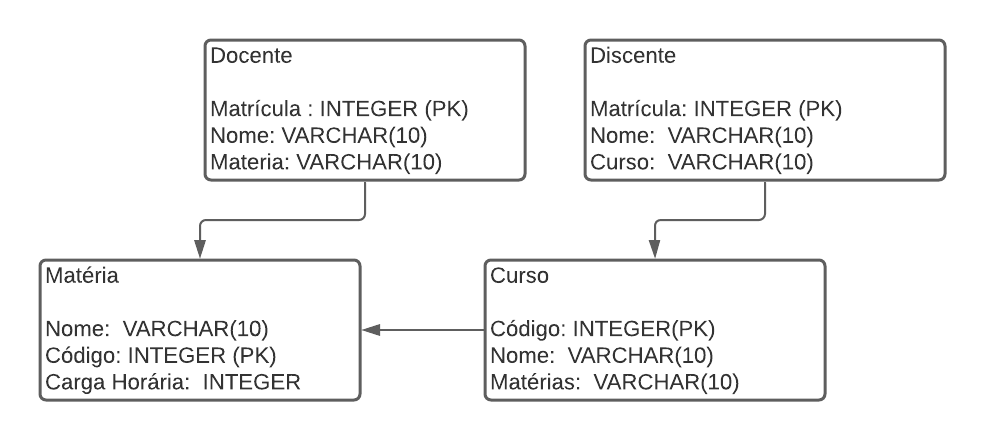
\includegraphics[width=.9\textwidth]{Modelo_Fisico.png}
\caption{Modelo físico.}
\label{fig:ModeloFisico}
\end{figure}

Também foi feito a base do sistema de banco de dados utilizando o utilitário do linux sqlite3 para fazer um arquivo SQLite com as tabelas apresentadas.

\begin{figure}[ht]
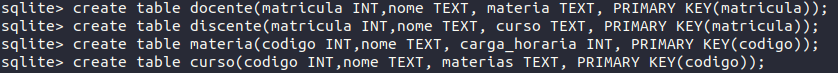
\includegraphics[width=1\textwidth]{criacao_tabelas.png}
\caption{Criacao tabelas.}
\label{fig:CriacaoTabela}
\end{figure}

\end{document}
